\documentclass[border=3pt]{standalone}
\usepackage{fontspec}
\newfontfamily\chessfont{Apple Symbols}
\usepackage{tikz}
\usepackage{pgfplots}
\pgfplotsset{compat=1.17}
\definecolor{light}{HTML}{EDEDED}
\definecolor{dark}{HTML}{7389B8}
\definecolor{edge}{HTML}{4A4A4A}
\definecolor{blue2}{HTML}{B9C6E0}
\begin{document}
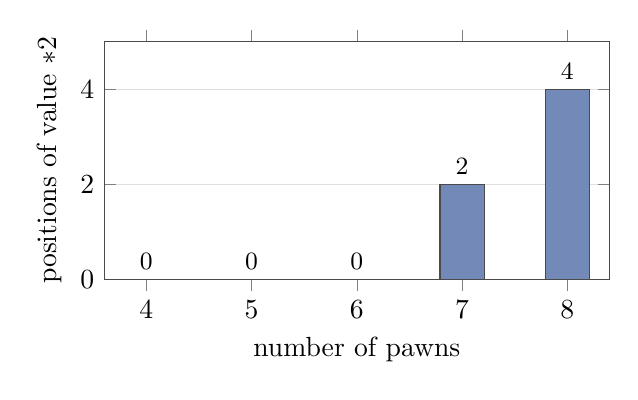
\begin{tikzpicture}\begin{axis}[ybar, bar width=16pt, width=8cm, height=4.6cm, ymin=0, ymax=5,
  xtick={4,5,6,7,8}, xlabel={number of pawns}, ylabel={positions of value $\ast2$},
  ymajorgrids, grid style={gray!25}, axis line style={edge}, nodes near coords,
  nodes near coords style={font=\small}]
\addplot[fill=dark, draw=edge] coordinates {(4,0) (5,0) (6,0) (7,2) (8,4)};
\end{axis}\end{tikzpicture}
\end{document}
